% LaTeX Poster vim:ts=2 sw=2
% 
\documentclass[final,hyperref={pdfpagelabels=false}]{beamer}
\mode<presentation>{\usetheme{I6pd2}}

\usepackage{grffile}
\usepackage[english]{babel}
\usepackage[latin1]{inputenc}
\usepackage{amsmath,amsthm, amssymb, latexsym}
\usepackage{algorithm,algorithmic}

\boldmath
\usepackage{graphicx}
\usepackage[orientation=portrait,size=a2,scale=1.4]{beamerposter}
% change list indention level
% \setdefaultleftmargin{3em}{}{}{}{}{}
%\usepackage{snapshot} % will write a .dep file with all dependencies, allows for easy bundling

\usepackage{array,booktabs,tabularx}
\newcolumntype{Z}{>{\centering\arraybackslash}X} % centered tabularx columns
\newcommand{\pphantom}{\textcolor{ta3aluminium}} % phantom introduces a vertical space in p formatted table columns??!!

%\listfiles

%%%%%%%%%%%%%%%%%%%%%%%%%%%%%%%%%%%%%%%%%%%%%%%%%%%%%%%%%%%%%%%%%%%%%%%%%%%%%%%%%%%%%%
\graphicspath{{figures/}}
% Section References
\newcommand{\secref}[1] {\hyperref[#1]{Section~\ref*{#1}}}
\newcommand{\eqnref}[1] {Equation \eqref{#1}}
\newcommand{\thmref}[1] {Theorem \ref{#1}}
\newcommand{\lmref}[1] {Lemma \ref{#1}}
\newcommand{\algoref}[1] {\hyperref[#1]{Algorithm~\ref*{#1}}}
%\renewcommand{\algorithmiccomment}[1]{\textit{// #1}}
%\theoremstyle{plain} \newtheorem{thm}{Theorem}

%Math Operators
\DeclareMathOperator {\argmax} {argmax}
\DeclareMathOperator {\sgn} {sgn}
\DeclareMathOperator {\trace} {tr}
\DeclareMathOperator{\E} {E}
\DeclareMathOperator{\Var} {Var}

\renewcommand{\Re} {\mathbb{R}}

\newcommand{\ud}{\, \mathrm{d}}
\newcommand{\diff}[1] {\frac{\partial}{\, \partial #1}}
\newcommand{\diffn}[2] {\frac{\partial^{#2}}{\, \partial {#1}^{#2}}}
\newcommand{\tuple}[1] {\langle #1 \rangle}

%Short hand
\newcommand{\mdp} {\ensuremath{\mathcal{M}}}
\newcommand{\states} {\mathcal{S}}
\newcommand{\actions} {\mathcal{A}}
\newcommand{\transitions} {\mathcal{P}}
\newcommand{\rewards} {\mathcal{R}}
\newcommand{\graph} {\mathcal{G}}
\newcommand{\policy} {\pi}
\newcommand{\initset} {\mathcal{I}}
\newcommand{\stopcond} {\beta}
\newcommand{\option} {\tuple{ \initset,\policy,\stopcond} }
\newcommand{\options} {\mathcal{O}}

%Math Operators
\DeclareMathOperator {\ball} {B}
\DeclareMathOperator {\ballf} {B^{f}}
\DeclareMathOperator {\sball} {b}
\DeclareMathOperator {\sballf} {b^{f}}

%Short hand
\newcommand{\arbcnst} {\tilde{c}}
\newcommand{\greedyalgo} {\ensuremath{\mathcal{GA}~}}

 
\title{Learning in a Small World}
\author{ Arun Tejasvi Chaganty \and Prateek Gaur \and Balaraman Ravindran \inst{1} } 
\institute[Indian Institute of Technology Madras]{ Reconfigurable and
Intelligent Systems Engineering Lab, \\ Deptt of Computer Science and
Engineering, \\ IIT Madras, Chennai, India - 600036 }
%\date[Sep. 8th, 2009]{Sep. 8th, 2009}

%%%%%%%%%%%%%%%%%%%%%%%%%%%%%%%%%%%%%%%%%%%%%%%%%%%%%%%%%%%%%%%%%%%%%%%%%%%%%%%%%%%%%%
% You wlll have to manually set the height of the page
% 105cm is good for A0. 52 for A2, 22 for A3
\newlength{\columnheight}
\setlength{\columnheight}{50cm}
%%%%%%%%%%%%%%%%%%%%%%%%%%%%%%%%%%%%%%%%%%%%%%%%%%%%%%%%%%%%%%%%%%%%%%%%%%%%%%%%%%%%%%
\begin{document}

% Everything is contained in this frame
\begin{frame}
  % Standard two column layout
  \begin{columns}
    %%%%%%%%%%%%%%%%%%%%%%%%%%%%%%%%%%%%%%%%%%%%%%%%%%%%%%%%%%%%%%%%%%%%%%%%%%%%%%%%%%%%%%
    % Column 1
    \begin{column}{.49\textwidth}
      \begin{beamercolorbox}[center,wd=\textwidth]{postercolumn}
        \begin{minipage}[T]{.95\textwidth}  % tweaks the width, makes a new \textwidth
          \parbox[t][\columnheight]{\textwidth}{ % must be some better way to set the the height, width and textwidth simultaneously
            % Since all columns are the same length, it is all nice and tidy.  You have to get the height empirically
            % ---------------------------------------------------------%
            % fill each column with content            
            \begin{block}{Introduction}
    \begin{itemize}
        \item How do we perform such a diverse set of complex tasks?
            \begin{itemize}              
                \item Given an MDP with options, $\mdp
                    \tuple{\states,\options,\transitions,\cdot}$, can we
                    quickly learn any task (i.e. different $\rewards$)?
            \end{itemize}
        \item Most literature focuses on finding options to reach `bottlenecks',
            which are common subgoals across tasks. The objective of these
            options is to aid in early exploration.
            \begin{itemize}              
                \item A. McGovern and A. G. Barto, ``Automatic Discovery of
                    Subgoals in Reinforcement Learning using Diverse Density,''
                    in ICML, 2001
                \item I. Menache, S. Mannor, and N. Shimkin, ``Q-Cut - Dynamic
                    Discovery of Sub-Goals in Reinforcement Learning,'' in ECML,
                    2002. 
                \item \"{O}. \c{S}im\c{s}ek and A. G. Barto, ``Skill
                    characterization based on betweenness,'' in NIPS, 2008 
            \end{itemize}              
        \item Our1 Hypothesis: The key is in finding a set of composable subtasks
            spanning the space of tasks.
    \end{itemize}              
\end{block}

\vfill
\begin{block}{Motivation: The Small World Phenomenon}
    \begin{itemize}
        \item Kleinberg: ``Individuals using local information are collectively
            very effective at actually constructing short paths between two
            points in a social network.'' \\
            {\small J. Kleinberg, ``The Small-World
            Phenomenon: An Algorithmic Perspective'' in ACM Theory of Computing,
            2000}
        \item Kleinberg constructed a family of networks for which the expected
            time to deliver a message from any source to any destination was
            $( \log |\mbox{size of network}| )^2$, using the inverse power law distribution.
            \begin{itemize}              
                \item Structural properties of the network are important
            \end{itemize}              
        \item Can we do the same for learning?
            \begin{itemize}              
                \item A {\bf small-world RL domain} has the property that an
                    agent using local information (e.g. the value function) can
                    effectively reach a state of {\em maximal value}.
            \end{itemize}              
    \end{itemize}
\end{block}

\vfill
\begin{block}{Generating Options according to $P_r$}
    \begin{columns}
        \begin{column}{.39\textwidth}
            \begin{figure}[h]
                \centering
                \includegraphics[height=3in]{figures/rooms-options}
                \label{fig:rooms-options}
                \caption{Some $P_2$ Options}
            \end{figure}
        \end{column}
        \begin{column}{.49\textwidth}                
            \begin{itemize}
                \item Consider the state-interaction graph of $\mdp$. 
                \item For each state $s \in \states$, select a single $s'$
                    reachable from $s$ according to the inverse power law
                    distribution $P_r : p(s,s') \propto \|s - s'\|^{-r}$.
                \item For each $(s,s')$ pair, construct an option $o:\option$
                    with $\initset = \{s\}$, $\stopcond = \{s'\}$, and $\pi =
                    \mbox{optimal policy to reach $s'$}$.
            \end{itemize}
        \end{column}
    \end{columns}

    {\em Note: This construction adds just one additional action for each state,
    and thus does not blow up the agent's search space.}

\end{block}

\vfill
\begin{block}{Theorem: $O( (\log n)^2 )$ Decisions}
    Assume $\mdp$ to have states arranged in a $k$-dimensional lattice, with
    noisy (with parameter $\epsilon$) primitive navigation actions $\actions$,
    and rewards distributed between $[0,1]$.

    Using only the value of neighboring states, an agent with options $\options$
    generated by $P_k$, can reach a state of maximal value in $O( ( \log
    |\states| )^2)$ decisions.

    \begin{itemize}
        \item We relate the value of two states $u$ and $v$, and their lattice distance,
            $$ \log \frac{ V(v) }{ V(u) } \approx \log( \sqrt{ \frac{1 - \epsilon}{ \epsilon } } ) \|u - v\| + c,$$ 
            where $c \in [0,\frac{1}{1-\gamma}]$.
        \item Following Kleinberg's analysis, we show that using the optimal
            value function, the agent makes $O(\log |\states|)$ decisions to get
            exponentially closer to the maximal value state. 
    \end{itemize}

\end{block}

          }
        \end{minipage}
      \end{beamercolorbox}
    \end{column}

    %%%%%%%%%%%%%%%%%%%%%%%%%%%%%%%%%%%%%%%%%%%%%%%%%%%%%%%%%%%%%%%%%%%%%%%%%%%%%%%%%%%%%%
    % Column 2
    \begin{column}{.49\textwidth}
      \begin{beamercolorbox}[center,wd=\textwidth]{postercolumn}
        \begin{minipage}[T]{.95\textwidth} % tweaks the width, makes a new \textwidth
          \parbox[t][\columnheight]{\textwidth}{ % must be some better way to set the the height, width and textwidth simultaneously
            % Since all columns are the same length, it is all nice and tidy.  You have to get the height empirically
            % ---------------------------------------------------------%
            % fill each column with content
            
\begin{block}{Results}
    \begin{figure}[h]
        \centering
        \fbox{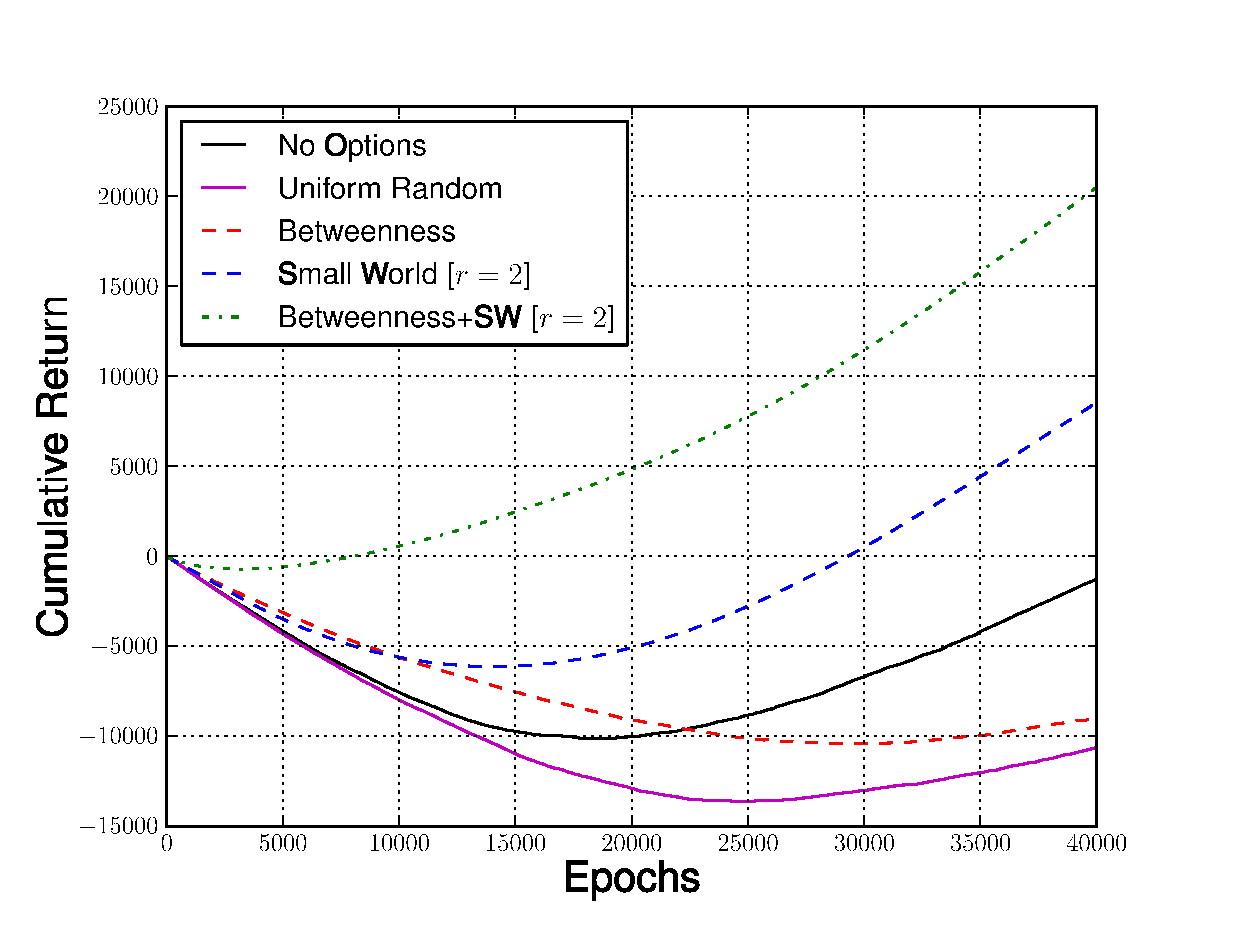
\includegraphics[height=4in]{figures/rooms-algos-200}}
        \label{fig:rooms-performance}
        \caption{Rooms: Cumulative Return (with 200 options)}
    \end{figure}

    \vskip-4ex
    % Table
    \begin{columns}
        \begin{column}{.45\textwidth}
            \begin{table}
              \centering
              \small
              \begin{tabular}{ l r r } %{@{} p{.25\linewidth} p{.2\linewidth} p{.2\linewidth} p{0.2\linewidth} }
                \toprule 
                Scheme & \multicolumn{2}{c @{}}{Options (40,000 epochs)}  \\
                \cmidrule(l){2-3}
                                & {200}             & {400}  \\
                \toprule
                None            & -31.82         & -31.82   \\
                \addlinespace                            
                $P_0$           & -31.23         & -32.90   \\  
                \addlinespace                            
                Betw.           & -18.28         & -24.38   \\
                \addlinespace                                  
                $P_4$           & {\bf -14.24}   & {\bf -7.55}    \\
                \bottomrule
              \end{tabular}
              \caption{Arb. Nav.: Cumulative Return}
            \end{table}
        \end{column}
        \begin{column}{.45\textwidth}                
            \begin{table}
              \centering
              \small
              \begin{tabular}{ l r r } %{@{} p{.25\linewidth} p{.2\linewidth} p{.2\linewidth} p{0.2\linewidth} }
                \toprule 
                Scheme & \multicolumn{2}{c @{}}{Options (40,000 epochs)}  \\
                \cmidrule(l){2-3}
                                        & {100}         & {200}            \\ %& {400}    \\
                \toprule                                    
                None                    & -16.90        & -16.90           \\ %& -3043.60 \\
                \addlinespace                                                   %          
                $P_0$                   & -17.68         & -18.83           \\ %& -8304.05 \\  
                \addlinespace                                                   %           
                Betw.                   & {\bf 80.59}   & {\bf 80.48}      \\ %& 14841.15 \\
                \addlinespace                                                   %   
                $P_{0.75}$                 & -7.55          & 0.66             \\ %& 22605.01 \\
                % \addlinespace                                                %     
                % Betw. + \\$P_{0.75}$      & 12.69          & 15.12        \\ %& {\bf 23168.17} \\
                \bottomrule
              \end{tabular}
              \caption{Taxi: Cumulative Return}
            \end{table}
        \end{column}
    \end{columns}

    % Comments
    \begin{itemize}
        \item Experiments were run for 40,000 epochs using MacroQ. We compared
            options generated using a bottleneck based method (betweenness),
            randomly distributed options ($P_0$), and small world options ($P_{r
            > 0}$).
        \item Bottleneck-based methods have a natural advantage in the Taxi
            domain, as goal states coincide with bottleneck states (the {\tt
            pick-up} and {\tt put-down} actions). 
        \item Small-world options do very well on free-navigation tasks (Rooms
            or Arbitrary Navigation), even in the presence of bottlenecks
            (Rooms). Combining bottleneck-based options and small world
            options can outperform both (Rooms).
    \end{itemize}
\end{block}

\vfill
\begin{block}{Role of the Exponent $r$ (Rooms)}
    \begin{columns}
        \begin{column}{.49\textwidth}
            \begin{figure}[h]
                \centering
                \fbox{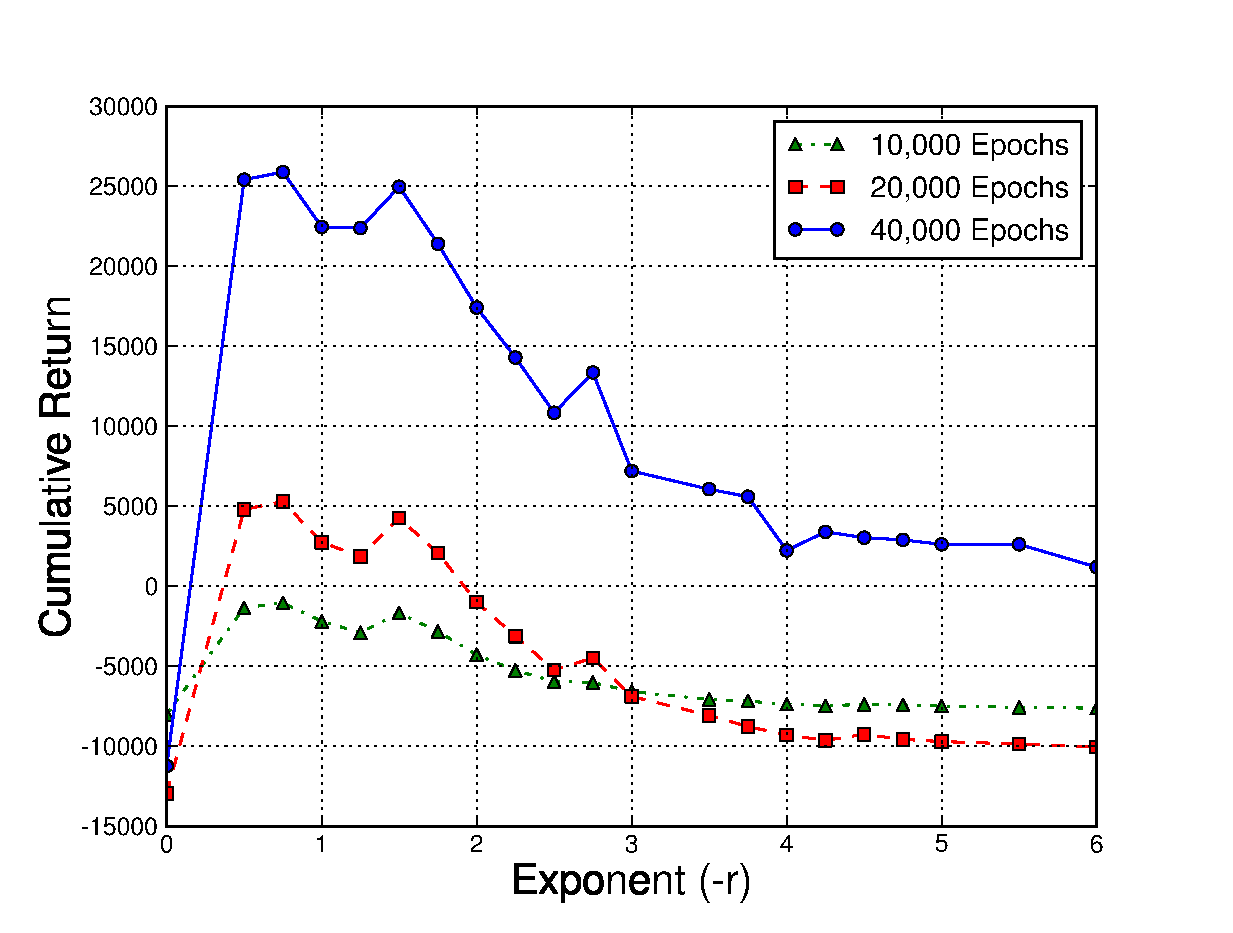
\includegraphics[height=3in]{figures/rooms-exp}}
                \label{fig:rooms-exponent}
                %\caption{Rooms}
            \end{figure}
        \end{column}
        \begin{column}{.39\textwidth}                
            \begin{itemize}
                \item The basic structure of the the Rooms state spaces is 2D,
                    yet exponents around 1 perform optimally.  This difference
                    is likely due to obstacles (walls).
                \item The existance of a maximal value for the exponent, as well
                    the behaviour for exponents greater than it, matches what is
                    seen in the social networks scenario.
            \end{itemize}
        \end{column}
    \end{columns}
\end{block}

\vfill
\begin{block}{Conclusions}
    \begin{itemize}
        \item We give an algorithm to generate a random collection of options
            $\options$ such that any ``task'' in an MDP can be performed in
            $O( ( \log |\states| )^2 )$ decisions.
        \item We find that these options significantly outperform
            bottleneck-based options and purely random options.
    \end{itemize}
\end{block}

\vfill
\begin{block}{Future Work}
    \begin{itemize}
        \item By using `cheaply' learnt policies could the total training time
            for small world options compare to say that for the case of
            betweenness?
        \item Given the loose conditions for the theorem to hold, could function
            approximators be used inplace of the complete MDP?
        \item Could the bounded number of decisions required translate to any
            theoretical guarantees on faster convergence?
    \end{itemize}
\end{block}

          }
          % ---------------------------------------------------------%
          % end the column
        \end{minipage}
      \end{beamercolorbox}
    \end{column}
    % ---------------------------------------------------------%
    % end the column
  \end{columns}
  \vskip2ex
\end{frame}

\end{document}

